\section{Dilema Sosial}

Dilema sosial merupakan situasi di mana keputusan rasional secara individual menghasilkan luaran yang tidak optimal secara kolektif(~\cite{axelrod_evolution_1981}). Secara formal, kondisi ini dapat dinyatakan sebagai:


\[\sum_{i=1}^{n} u_i(a_i, a_{-i}) 
<
\sum_{i=1}^{n} u_i(a'_i, a'_{-i})\]


di mana $n$ adalah jumlah pemain,$u_i$ adalah fungsi utilitas pemain $i$, $a_i$ adalah aksi rasional individu dan $a'_i$ adalah profil aksi yang memaksimalkan kesejahteraan kolektif.

Formulasi ini menjelaskan adanya konflik antara rasionalitas individu dan optimalitas sosial. Namun, ekspresi agregat tersebut belum menyediakan struktur analitis yang cukup untuk memodelkan interaksi strategis antar agen secara eksplisit.


\section{Game Theory}

teori permainan memberikan kerangka formal yang memodelkan pemain, strategi, dan payoff secara terstruktur (\cite{bonanno_game_2024}), dalam bentuk normal didefinisikan sebagai:

\[G = (N, A, U)\]

dengan $N$ himpunan pemain, $A = A_1 \times A_2$ himpunan profil strategi atau \textit{Action space }, dan $U = (u_1, u_2)$ fungsi payoff atau\textit{utility}.

\textit{Nash Equilibrium} adalah profil strategi $a^*$ yang memenuhi:

\[
u_i(a_i^*, a_{-i}^*) \ge u_i(a_i, a_{-i}^*)
\quad \forall a_i \in A_i
\]

Menunjukan pilihan aksi selain $a_i^*$ tidak dapat memberikan keuntungan lebih besar dari strategi keseimbangan. Kerangka ini memungkinkan analisis rasionalitas strategis dalam interaksi statik. Namun, model bentuk normal bersifat satu tahap dan mengasumsikan struktur payoff tetap. 

\section{Prisoner's Dilemma}\label{sec:PrisonersDilemma}

Prisoner's Dilemma merepresentasikan konflik rasionalitas individu dan kolektif secara eksplisit (~\cite{axelrod_evolution_1981}). Aksi yang dapat dipilih adalah \textit{Cooperate} ($C$) atau \textit{Defect} ($D$). Struktur payoff Prisoner's Dilemma diberikan oleh:


\begin{table}[h]
\centering
\begin{tabular}{c|cc}
    & C & D \\
\hline
C & $(R,R)$ & $(S,T)$ \\
D & $(T,S)$ & $(P,P)$
\end{tabular}
\caption{Payoff Matrix Prisoner's Dilemma}
\end{table}

Dengan $R$ (Reward) adalah payoff jika kedua pemain bekerja sama, $T$ (Temptation) adalah payoff bagi pemain yang berkhianat sementara yang lain bekerja sama, $S$ (Sucker's payoff) adalah payoff bagi pemain yang bekerja sama sementara yang lain berkhianat, dan $P$ (Punishment) adalah payoff jika kedua pemain berkhianat.
dengan ketidaksamaan:

\[
T > R > P > S
\quad \text{dan} \quad
2R > T + S .
\]

Dalam permainan satu tahap, strategi dominan adalah defeksi ($D$), sehingga keseimbangan Nash berada pada $(D,D)$ meskipun $(C,C)$ lebih optimal secara kolektif. Namun, interaksi nyata jarang terjadi hanya satu kali. 

\section{Prisoner's Dilemma Berulang}\label{sec:IPD}

Permainan PD diperluas menjadi bentuk berulang disebut Iterated Prisoner's Dilemma (IPD), permainan diulang selama $T$ atau \textit{Turn} tahap dengan payoff kumulatif atau terdiskonto. Dalam IPD, strategi dapat bergantung pada histori interaksi, memungkinkan untuk pembalasan dan kerja sama yang berkelanjutan. IPD relevan untuk mempelajari dinamika manusia seperti: pembentukan hubungan, konflik berkepanjangan, siklus saling membalas, dan pemulihan kepercayaan.

berberapa strategi terkenal dalam IPD meliputi:
\begin{itemize}
    \item \textit{Tit-for-Tat}: Mulai dengan bekerja sama, kemudian meniru aksi lawan pada langkah sebelumnya.
    \item \textit{Cooperator}: Selalu bekerja sama.
    \item \textit{Defector}: Selalu berkhianat.
    \item \textit{Random}: Memilih secara acak antara bekerja sama dan berkhianat.
\end{itemize}

beberapa algoritma tersebut dapat dipahami melalui gambar \ref{fig:dfa} finite state machine.

\begin{figure}[!htbp]
    \centering
    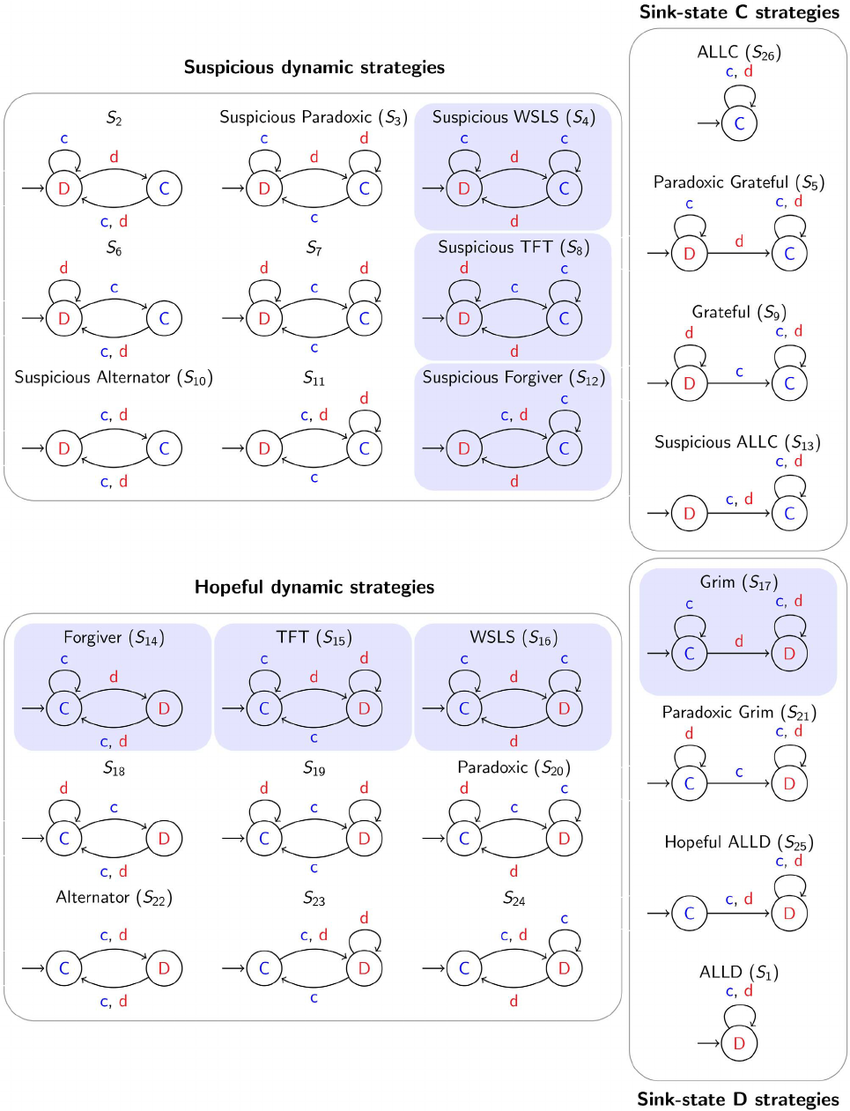
\includegraphics[height=0.8\textheight]{Images/dfa.png}
    \caption{Finite Automata untuk strategi IPD \cite{reiter_deterministic_strategies_2014}}\label{fig:dfa}
\end{figure}


\subsection{Horizon Terbatas}

Pada formulasi horizon terbatas dengan panjang permainan tetap $T$, utilitas total pemain didefinisikan sebagai penjumlahan utilitas pada setiap ronde:

\begin{equation}
U_i = \sum_{t=1}^{T} u_i(a_i^t, a_{-i}^t)
\end{equation}

Pada model ini, tidak digunakan faktor diskonto. Namun, secara teoretis, pendekatan ini cenderung menghasilkan strategi defeksi melalui mekanisme \textit{backward induction} (\cite{bonanno_game_2024}).

\subsection{Definisi Riwayat Interaksi pada mekanisme online}

Dalam konteks iterated game dua pemain, riwayat hingga waktu $t$ tidak hanya terdiri dari aksi satu pemain, tetapi pasangan aksi kedua pemain pada setiap putaran. 
Secara formal, riwayat didefinisikan sebagai:

\[
H_t = \left( (a_i^1, a_{-i}^1), (a_i^2, a_{-i}^2), \dots, (a_i^t, a_{-i}^t) \right)
\]

dengan $a_i^k$ menyatakan aksi pemain $i$ pada waktu $k$, dan $a_{-i}^k$ menyatakan aksi lawan pada waktu yang sama.

Dalam pengaturan iteratif, riwayat tidak tersedia secara sekaligus, melainkan terbentuk secara \textit{online} (\cite{bonanno_game_2024}). Pada setiap putaran $t$, riwayat diperbarui secara inkremental sebagai:

\[
H_t = (H_{t-1}, (a_i^t, a_{-i}^t))
\]

dengan $H_0 = \emptyset$.

Formulasi ini menegaskan bahwa agen tidak memiliki akses terhadap trajektori interaksi di masa depan, dan hanya dapat menggunakan informasi yang telah terobservasi hingga waktu berjalan. Dengan kata lain, proses pengambilan keputusan berlangsung dalam kerangka kausal dan sekuensial (\cite{bonanno_game_2024}).

riwayat interaksi menyediakan rekaman lengkap atas realisasi aksi kedua pemain. \textit{Namun}, riwayat hanya merepresentasikan keluaran observabel dari proses pengambilan keputusan lawan, bukan mekanisme generatif yang mendasarinya. Agen tidak memiliki akses langsung terhadap strategi internal, parameter keputusan, ataupun aturan adaptasi yang digunakan oleh lawan (\cite{bonanno_game_2024}).

Dengan demikian, meskipun seluruh pasangan aksi teramati secara bertahap, struktur strategi lawan tetap bersifat laten. Kondisi ini menyebabkan interaksi dalam IPD tidak memenuhi asumsi informasi lengkap sebagaimana pada analisis keseimbangan statik klasik (\cite{bonanno_game_2024}).

Oleh karena itu, permasalahan strategis dalam IPD dengan agen adaptif berada dalam kerangka permainan dengan informasi tidak lengkap, di mana agen harus melakukan inferensi terhadap strategi lawan secara bertahap seiring pertambahan riwayat (\cite{bonanno_game_2024}).


\subsection{Informasi tidak lengkap dan Pembentukan kepercayaan}

Dalam permainan dengan informasi tidak lengkap, ketidakpastian terhadap strategi lawan direpresentasikan melalui distribusi probabilitas atas kemungkinan tipe atau parameter strategi. Alih-alih mengasumsikan strategi tetap dan diketahui, agen memelihara suatu state kepercayaan yang diperbarui seiring bertambahnya histori interaksi.

Secara konseptual, state kepercayaan pada waktu $t$ dapat dituliskan sebagai:
\[
b_t = P(\theta \mid h_t)
\]
dengan $\theta$ merepresentasikan representasi laten dari strategi lawan, dan $h_t$ adalah histori interaksi hingga waktu $t$.

Formulasi ini menegaskan bahwa pengambilan keputusan dalam IPD adaptif bukan sekadar persoalan memilih aksi optimal terhadap strategi tetap, melainkan proses pembaruan kepercayaan secara sekuensial terhadap dinamika perilaku lawan. Dengan demikian, fokus analisis bergeser dari pencarian equilibrium statik menuju inferensi dinamis berbasis histori (\cite{bonanno_game_2024}).

\section{Pemodelan Lawan}

Pemodelan lawan memungkinkan untuk mempelajari perilaku ataupun strategi lawan (\cite{shoham_multiagent_2009}). 

Diberikan riwayat interaksi penuh:

\begin{equation}
h_t = \left( (a_i^1, a_{-i}^1), \dots, (a_i^t, a_{-i}^t) \right)
\end{equation}

model parametrik $f_\theta$ mempelajari distribusi kondisional:

\[p_\theta(a_{t+1}^{-i} \mid h_t)\]

Pendekatan regresi linear sederhana mampu memodelkan hubungan statik, namun memiliki keterbatasan dalam menangkap dependensi temporal dan pola nonlinier (\cite{hochreiter_long_1997}).

\section{Long Short-Term Memory (LSTM)}

Long Short-Term Memory (LSTM) merupakan pengembangan dari Recurrent Neural Network (RNN) yang dirancang untuk menangkap dependensi jangka panjang melalui mekanisme memori eksplisit (\cite{hochreiter_long_1997}). Dalam konteks pemodelan lawan, LSTM digunakan untuk membangun representasi laten terhadap strategi lawan berdasarkan histori interaksi.

Diberikan input $x_t$ (observasi pada waktu $t$, misalnya aksi lawan), hidden state sebelumnya $h_{t-1}$ (representasi laten sebelumnya), dan parameter bobot $W$, $U$, serta bias $b$, setiap komponen LSTM bekerja secara berurutan dengan ilustrasi gambar \ref{fig:LSTM}.

\begin{figure}[!htbp]
    \centering
    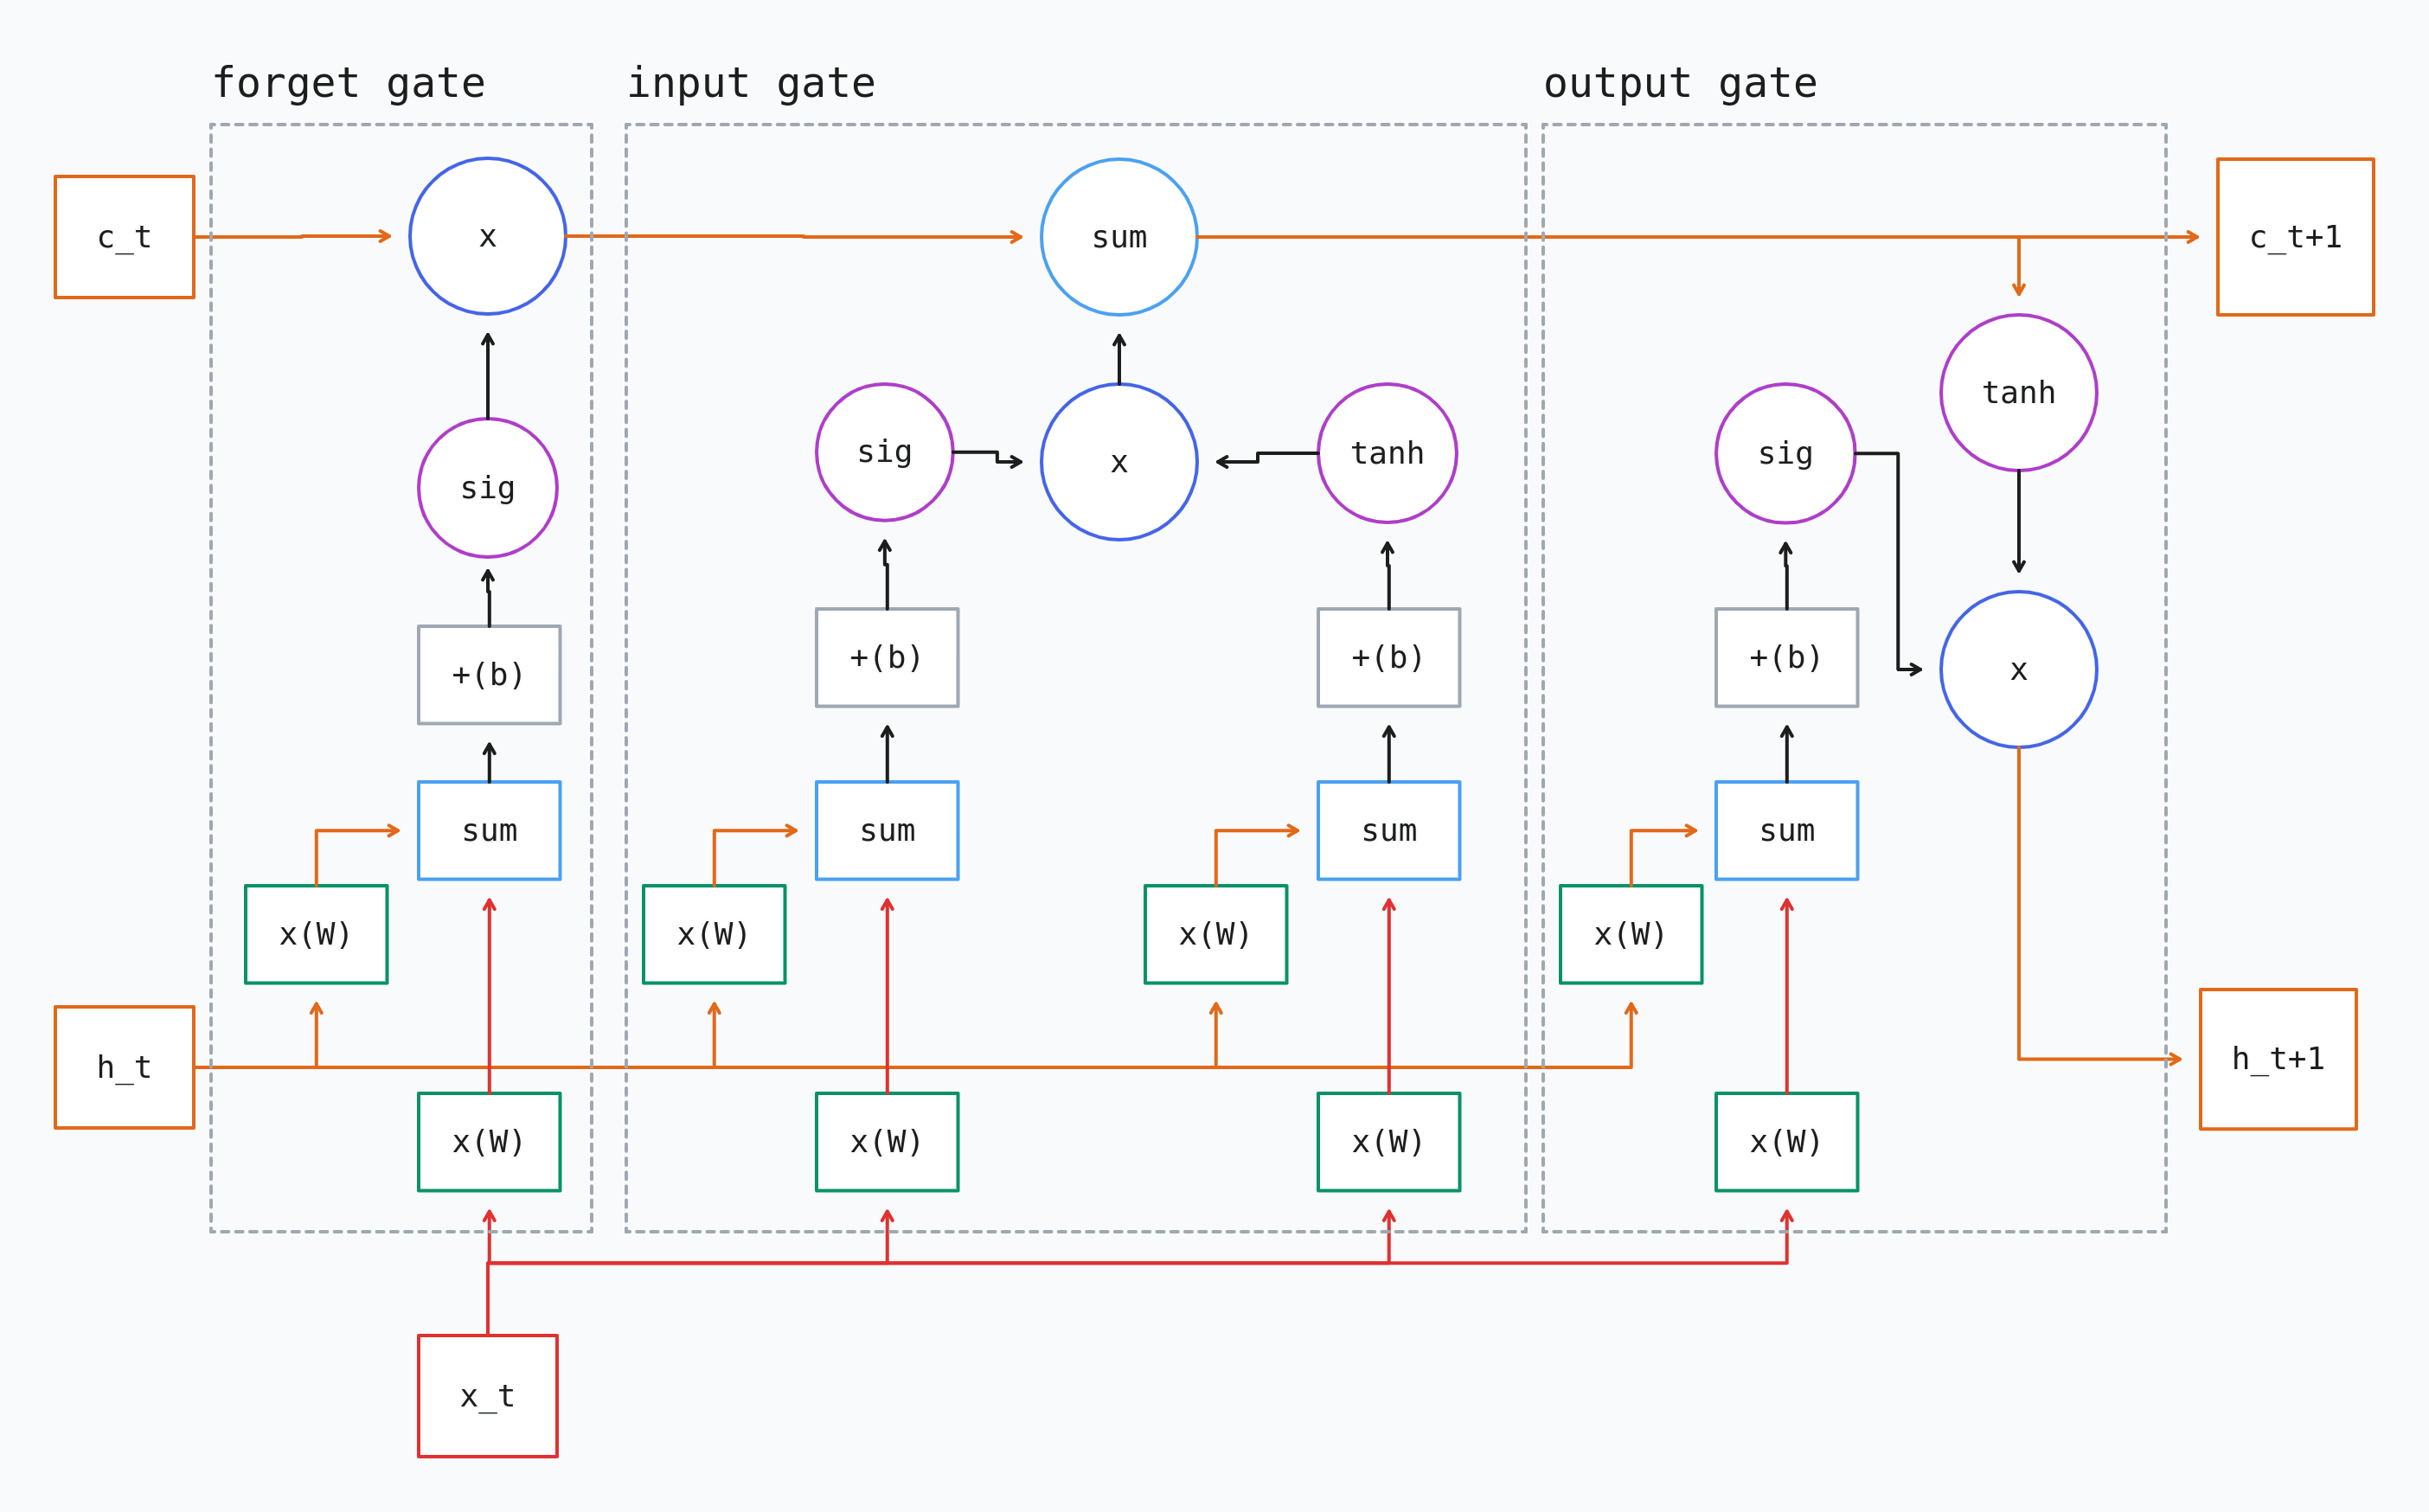
\includegraphics[height=0.4\textheight]{Images/LSTM.png}
    \caption{Diagram LSTM.}\label{fig:LSTM}
\end{figure}

\subsection{Forget Gate}

Forget gate mengontrol sejauh mana informasi pada state memori sebelumnya dipertahankan atau diabaikan pada waktu $t$ (\cite{hochreiter_long_1997}). Secara formal, nilai gerbang pelupaan $f_t$ dihitung melalui fungsi aktivasi sigmoid terhadap kombinasi linear antara input saat ini $x_t$, hidden state sebelumnya $h_{t-1}$, serta bias $b_f$. Parameter $W_f$ dan $U_f$ masing-masing merepresentasikan matriks bobot yang memetakan input dan hidden state ke ruang gerbang. Karena fungsi sigmoid menghasilkan keluaran pada rentang $(0,1)$, setiap elemen dalam $f_t$ berperan sebagai koefisien penskalaan yang mengatur proporsi informasi dari cell state sebelumnya yang akan dipertahankan. Nilai yang mendekati $1$ menunjukkan bahwa informasi tersebut dipertahankan hampir sepenuhnya, sedangkan nilai yang mendekati $0$ menyebabkan informasi tersebut dilupakan. Dengan demikian, forget gate memungkinkan model menyesuaikan horizon memori secara adaptif, sehingga dependensi temporal jangka panjang dapat dipertahankan atau dihapus sesuai kebutuhan dinamika data.
\begin{equation}
f_t = \sigma(W_f x_t + U_f h_{t-1} + b_f)
\end{equation}

\subsection{Input Gate}

Input $x_t \in \mathbb{R}^d$ merepresentasikan observasi saat ini, sedangkan $h_{t-1} \in \mathbb{R}^h$ adalah ringkasan historis interaksi sebelumnya (\cite{hochreiter_long_1997}). Namun, tidak semua informasi baru relevan atau stabil untuk memperbarui kepercayaan terhadap strategi lawan. Oleh karena itu, input gate $i_t \in [0,1]^h$ mengontrol seberapa besar setiap dimensi informasi baru akan diterima ke dalam memori, dengan $\sigma(\cdot)$ sebagai fungsi sigmoid dan $W_i, U_i, b_i$ sebagai parameter yang dipelajari.

\begin{equation}
i_t = \sigma(W_i x_t + U_i h_{t-1} + b_i)
\end{equation}


\subsection{Candidate Cell State}

Informasi mentah dari $x_t$ tidak langsung disimpan karena dapat mengandung noise atau pola sementara yang belum representatif (\cite{hochreiter_long_1997}). Namun, model tetap membutuhkan representasi kandidat dari informasi baru tersebut. Oleh karena itu, $\tilde{c}_t \in [-1,1]^h$ dibentuk melalui transformasi non-linear $\tanh(\cdot)$ sebagai kandidat memori baru, dengan parameter $W_c, U_c, b_c$.

\begin{equation}
\tilde{c}_t = \tanh(W_c x_t + U_c h_{t-1} + b_c)
\end{equation}

\subsection{Cell State (Memori Jangka Panjang)}

Cell state $c_t \in \mathbb{R}^h$ merupakan jalur utama propagasi informasi jangka panjang dalam LSTM (\cite{hochreiter_long_1997}) yang berfungsi sebagai \textit{latent kepercayaan representation} terhadap strategi lawan. Namun, memori ini harus mampu menjaga stabilitas sekaligus tetap adaptif terhadap informasi baru. Oleh karena itu, pembaruannya dirumuskan sebagai:

\begin{equation}
c_t = f_t \odot c_{t-1} + i_t \odot \tilde{c}_t
\end{equation}

Operator $\odot$ menyatakan perkalian elemen-per-elemen. Komponen $f_t \odot c_{t-1}$ mempertahankan informasi lama yang masih relevan, sedangkan $i_t \odot \tilde{c}_t$ menambahkan informasi baru secara selektif. Struktur aditif ini penting karena menjaga stabilitas gradien dan memungkinkan pembelajaran dependensi jangka panjang.

\subsection{Output Gate}

Meskipun $c_t$ menyimpan informasi lengkap, tidak seluruhnya relevan untuk prediksi saat ini. Namun, model perlu mengekstrak bagian informasi yang paling informatif untuk pengambilan keputusan (\cite{hochreiter_long_1997}). Oleh karena itu, output gate $o_t \in [0,1]^h$ mengontrol seberapa besar informasi dari cell state akan diekspos ke hidden state, dengan parameter $W_o, U_o, b_o$.

\begin{equation}\label{output_Gate}
o_t = \sigma(W_o x_t + U_o h_{t-1} + b_o)
\end{equation}

Pada persamaan di~\ref{output_Gate}, $x_t \in \mathbb{R}^{d}$ menyatakan vektor input pada waktu $t$ dengan dimensi fitur $d$, sedangkan $h_{t-1} \in \mathbb{R}^{h}$ adalah hidden state pada waktu sebelumnya dengan dimensi laten $h$. Matriks bobot $W_o \in \mathbb{R}^{h \times d}$ memetakan input ke ruang gerbang keluaran, dan $U_o \in \mathbb{R}^{h \times h}$ memetakan hidden state sebelumnya ke ruang yang sama. Vektor bias $b_o \in \mathbb{R}^{h}$ memungkinkan pergeseran afine dalam transformasi linear tersebut. Fungsi aktivasi sigmoid $\sigma(\cdot)$ diterapkan secara elemen-per-elemen sehingga menghasilkan $o_t \in (0,1)^h$, yaitu vektor koefisien yang mengatur proporsi informasi dari cell state $c_t$ yang akan diekspos ke hidden state saat ini. Dengan demikian, output gate berperan sebagai mekanisme penyaringan adaptif yang menentukan komponen representasi memori internal yang relevan untuk menghasilkan representasi laten $h_t$ dan prediksi pada waktu $t$.

\subsection{Hidden State Update}

Cell state $c_t$ mengandung representasi lengkap jangka panjang, namun terlalu kaya untuk digunakan secara langsung (\cite{hochreiter_long_1997}). Oleh karena itu, hidden state $h_t \in \mathbb{R}^h$ dibentuk sebagai representasi laten terfilter yang lebih terfokus, yang kemudian digunakan untuk memprediksi aksi lawan atau sebagai input ke modul pengambilan keputusan.

\begin{equation}
h_t = o_t \odot \tanh(c_t)
\end{equation}

Struktur ini memungkinkan model mempertahankan dependensi jangka panjang sekaligus tetap adaptif terhadap perubahan strategi lawan. Oleh karena itu, LSTM sangat sesuai untuk digunakan dalam permainan berulang seperti Iterated Prisoner's Dilemma, di mana perilaku lawan bergantung pada histori is`nteraksi. Namun, karena LSTM hanya menghasilkan prediksi satu langkah ke depan, model ini belum secara eksplisit mempertimbangkan konsekuensi jangka panjang, sehingga masih berpotensi menghasilkan kebijakan yang suboptimal.

\section{Prediksi Multi-Langkah}

Model LSTM menghasilkan distribusi prediktif satu langkah ke depan
$p(a_{t+1}^{-i} \mid h_t)$.
Namun, dalam permainan berulang,
nilai suatu aksi tidak hanya ditentukan oleh respons lawan pada tahap berikutnya,
melainkan oleh konsekuensi jangka panjang sepanjang lintasan interaksi (\cite{nashed_survey_2022}).

\subsection{Peramalan Rekursif dan Simulasi Monte Carlo (Horizon Tetap)}

Untuk memperoleh estimasi lintasan masa depan sepanjang horizon tetap $H$, 
model perilaku lawan digunakan secara autoregresif. 
Pada setiap langkah ke-$h$, prediksi aksi lawan dihasilkan dari distribusi:

\[
\hat{a}_{t+h}^{-i}
\sim
p_\theta(\cdot \mid \hat{H}_{t+h-1}),
\quad h = 1, \dots, H
\]

Pada formulasi di atas, $t$ menyatakan waktu keputusan saat ini, sedangkan $H \in \mathbb{N}$ adalah horizon prediksi tetap yang menentukan panjang lintasan masa depan yang dipertimbangkan. Indeks $h$ merepresentasikan langkah prediksi ke-$h$ relatif terhadap waktu $t$. Simbol $\hat{a}_{t+h}^{-i}$ menyatakan aksi lawan yang diprediksi pada waktu $t+h$, dengan superskrip $-i$ menunjukkan pemain lawan terhadap agen $i$. Distribusi prediktif $p_\theta(\cdot \mid \hat{H}_{t+h-1})$ merupakan model parametrik dengan parameter $\theta$ yang mengaproksimasi probabilitas aksi lawan bersyarat pada riwayat yang tersedia. Notasi $\hat{H}_{t+h-1}$ menyatakan riwayat interaksi yang telah diperluas secara rekursif hingga waktu $t+h-1$, termasuk aksi-aksi yang sebelumnya diprediksi atau direalisasikan selama proses rollout.

Proses ini menghasilkan distribusi atas lintasan aksi sepanjang horizon terbatas:


\[\hat{\tau}_{t}^{(H)} =
\left\{
\hat{a}_{t+1}^{-i},
\hat{a}_{t+2}^{-i},
\dots,
\hat{a}_{t+H}^{-i}
\right\}
\]

Lintasan prediksi sepanjang horizon $H$ dinotasikan sebagai $\hat{\tau}_{t}^{(H)}$, yaitu himpunan berurutan dari aksi lawan yang diproyeksikan mulai dari $t+1$ hingga $t+H$. Karena ruang kemungkinan lintasan bertumbuh secara eksponensial terhadap $H$, ekspektasi nilai tidak dihitung secara tertutup, melainkan didekati melalui simulasi Monte Carlo.


Karena jumlah kemungkinan lintasan tumbuh secara eksponensial terhadap $H$, 
ekspektasi payoff tidak dihitung secara analitik, 
melainkan diaproksimasi menggunakan simulasi Monte Carlo.

Untuk suatu aksi awal $a_t$, estimasi nilai diperoleh melalui $M$ simulasi independen:

\begin{equation}
\hat{Q}_H(a_t)
=
\frac{1}{M}
\sum_{m=1}^{M}
\sum_{k=0}^{H-1}
u_i^{(m)}(a_i^{t+k}, a_{-i}^{t+k})
\end{equation}

dengan:
\begin{itemize}
\item $H$ : horizon prediksi tetap,
\item $M$ : jumlah rollout Monte Carlo,
\item $u_i^{(m)}$ : payoff agen pada simulasi ke-$m$.
\end{itemize}

Karena horizon bersifat terbatas, faktor diskonto tidak diperlukan, 
dan nilai aksi merepresentasikan akumulasi payoff sepanjang jendela prediksi tetap.

Dengan demikian, evaluasi aksi dilakukan melalui aproksimasi ekspektasi 
atas distribusi lintasan terbatas, 
yang sepenuhnya ditentukan oleh model kepercayaan dan horizon yang telah ditetapkan.


\subsection{Teacher Forcing}

Pada model sekuens autoregresif seperti RNN atau LSTM,
prediksi pada waktu $t$ bergantung pada output pada waktu sebelumnya.
Dinamika umum model dapat dituliskan sebagai:

\[
h_t = f(h_{t-1}, y_{t-1}; \theta),
\]

\[
\hat{y}_t = g(h_t; \theta),
\]

dengan:
\begin{itemize}
    \item $h_t$ : hidden state pada waktu $t$,
    \item $y_{t-1}$ : input autoregresif pada waktu sebelumnya,
    \item $\hat{y}_t$ : prediksi model pada waktu $t$,
    \item $\theta$ : parameter model yang dipelajari.
\end{itemize}

Dalam skema \textit{teacher forcing}, selama proses pelatihan,
input autoregresif tidak berasal dari prediksi model,
melainkan digantikan oleh nilai ground-truth $y_{t-1}^{*}$.
Dengan demikian, dinamika pelatihan menjadi:

\[
h_t = f(h_{t-1}, y_{t-1}^{*}; \theta).
\]

Fungsi kerugian didefinisikan sebagai:

\begin{equation}
\mathcal{L}(\theta)
=
\sum_{t=1}^{T}
\ell(\hat{y}_t, y_t^{*}),
\end{equation}

dengan:
\begin{itemize}
    \item $T$ : panjang sekuens pelatihan,
    \item $\ell(\hat{y}_t, y_t^{*})$ : fungsi loss (misalnya cross-entropy atau MSE) 
    yang mengukur selisih antara prediksi dan target sebenarnya.
\end{itemize}

Teacher forcing mempercepat konvergensi
dan menghasilkan estimasi gradien yang lebih stabil,
karena distribusi input selama pelatihan
sesuai dengan distribusi data observasi.


\begin{figure}[!htbp]
    \centering
    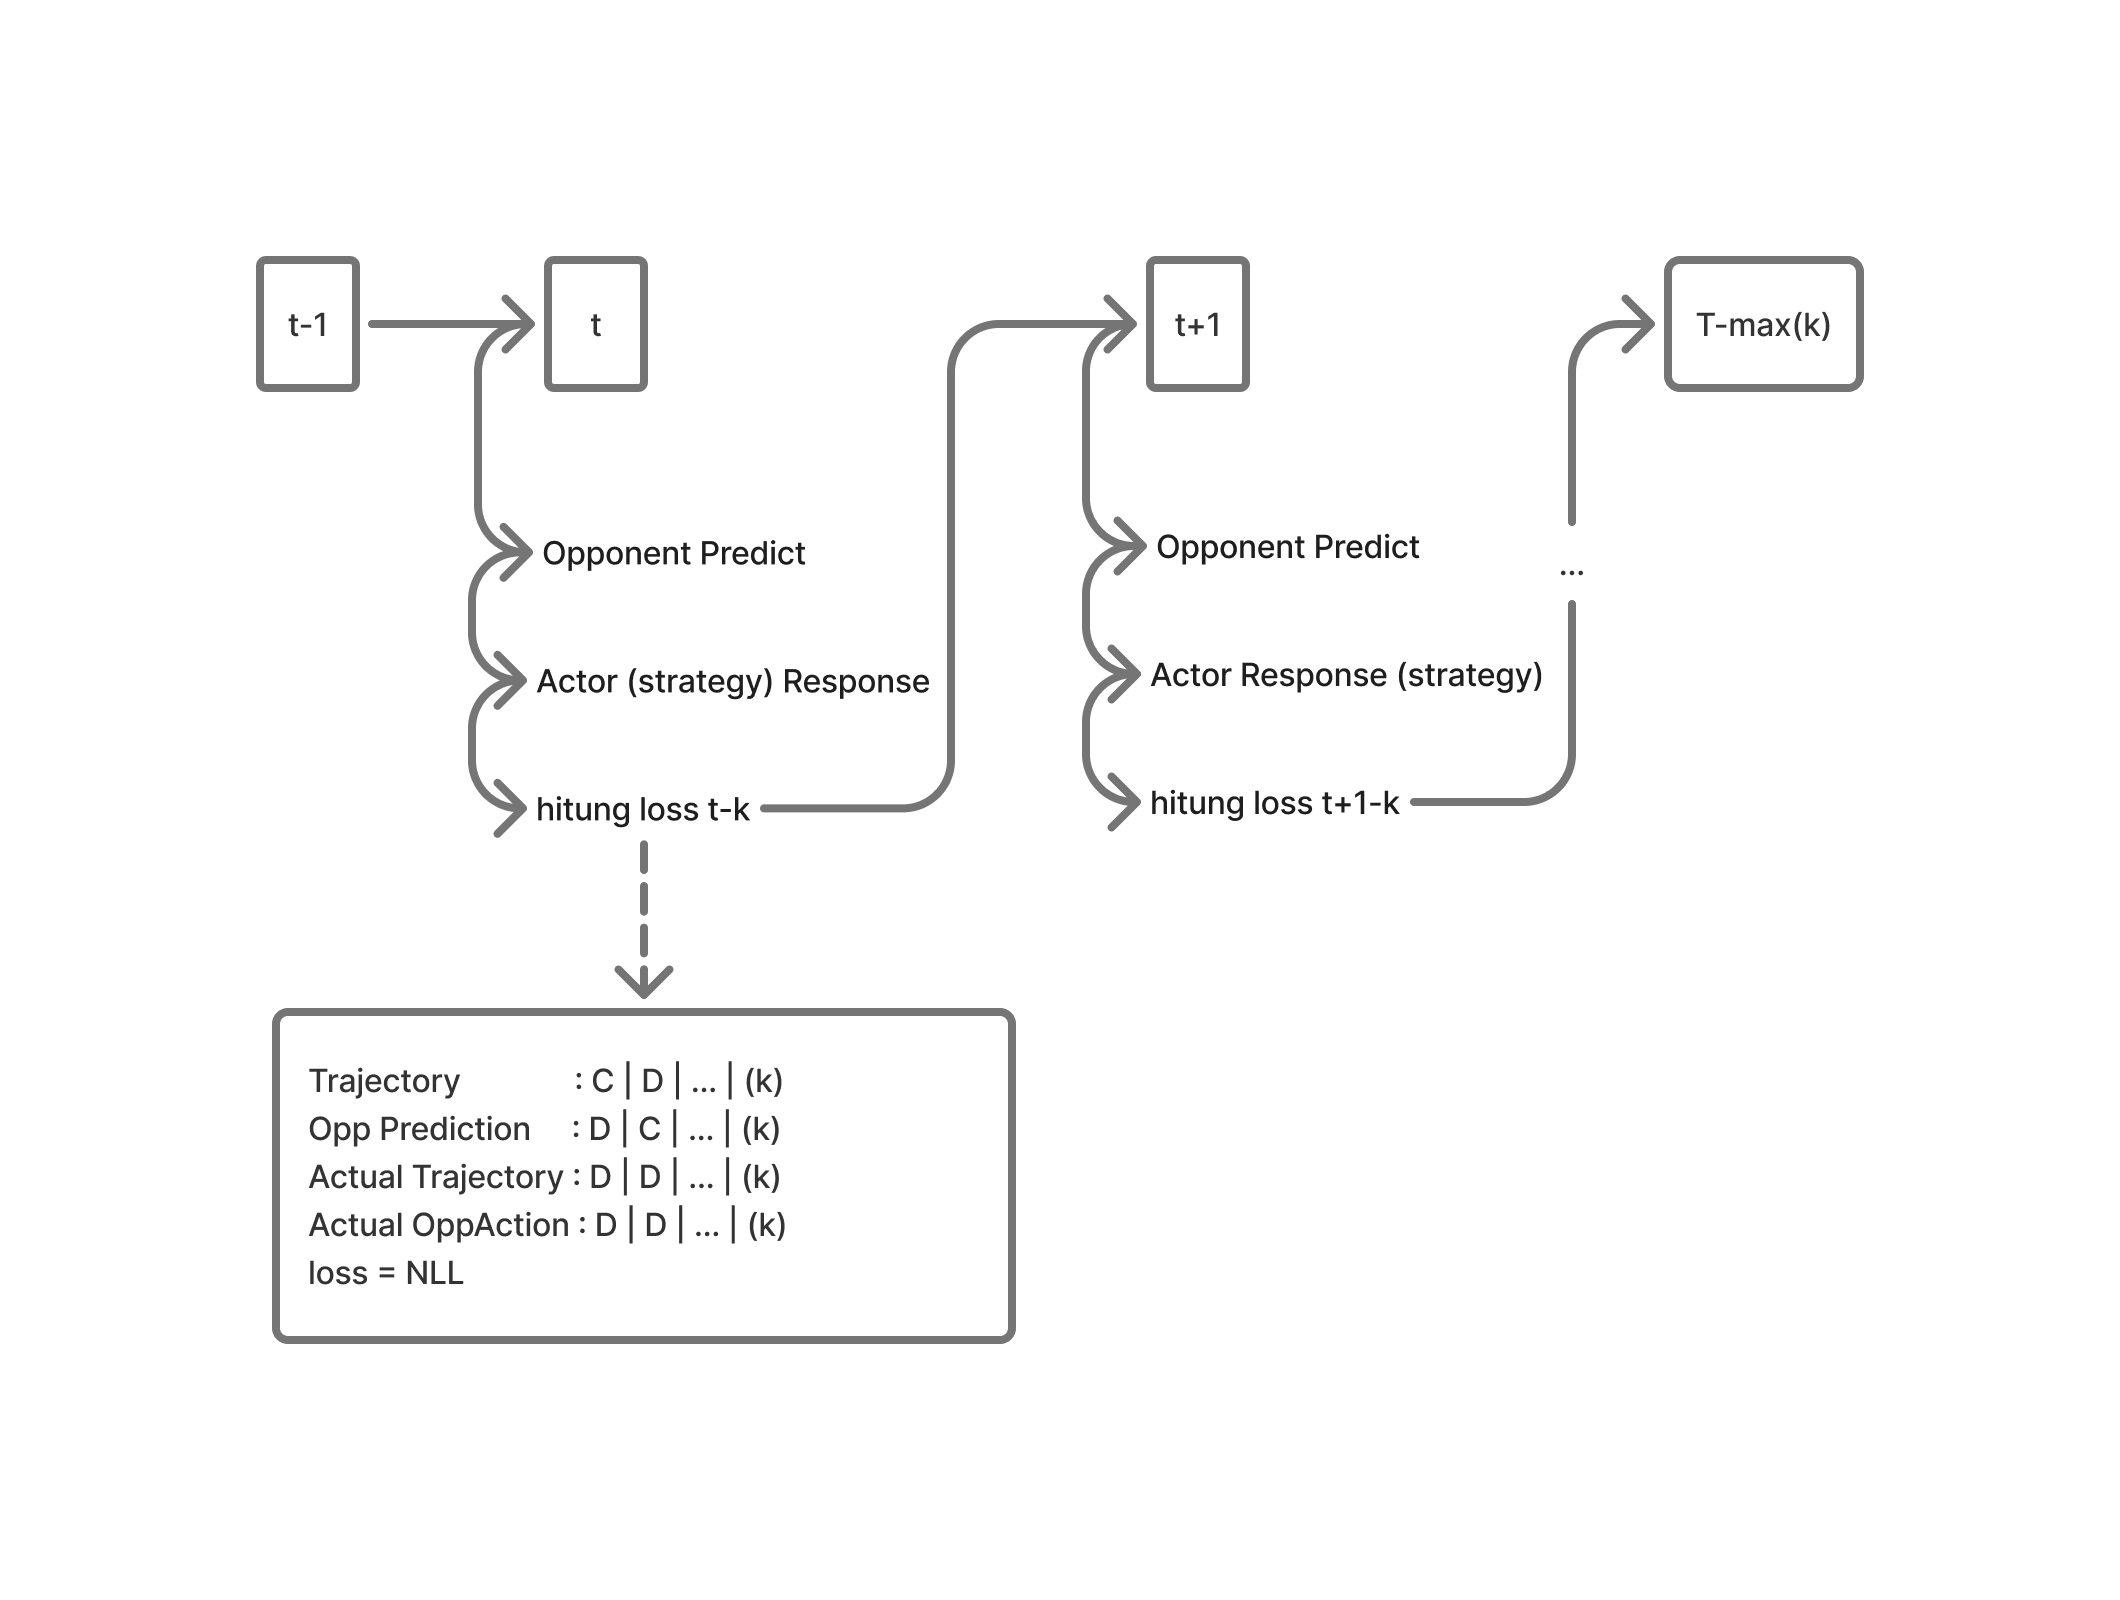
\includegraphics[width=0.9\textwidth]{Images/teacherForcing.png}
    \caption{Teacher Forcing.}\label{fig:teacherForcing}
\end{figure}

Namun, pada fase inferensi (deployment),
model tidak lagi memiliki akses ke ground-truth.
Prediksi harus dihasilkan secara rekursif menggunakan output sebelumnya:

\[
h_t = f(h_{t-1}, \hat{y}_{t-1}; \theta).
\]

Perbedaan antara distribusi input saat pelatihan
(menggunakan $y_{t-1}^{*}$)
dan saat inferensi
(menggunakan $\hat{y}_{t-1}$)
menimbulkan fenomena yang dikenal sebagai \textit{exposure bias}.
Akibatnya, kesalahan kecil pada satu langkah
dapat terpropagasi dan terakumulasi,
menyebabkan \textit{compounding error}
yang semakin signifikan pada horizon prediksi yang panjang.

\subsection{Fungsi Objektif Negative Log-Likelihood}

Untuk mengevaluasi kualitas prediksi sekuensial lawan dalam horizon 
multi-step, digunakan metrik \textit{Negative Log-Likelihood} (NLL) 
sebagai proper scoring rule yang konsisten terhadap estimasi distribusi probabilistik (\cite{zhu_negative_2018}).

Misalkan pada waktu $t$ tersedia riwayat interaksi 

\[
h_t = \{(a_i^1, a_{-i}^1), \dots, (a_i^t, a_{-i}^t)\}.
\]

Model pemodelan lawan menghasilkan distribusi probabilitas atas aksi lawan pada langkah berikutnya, yang dinotasikan sebagai:

\[
P_\theta(a_{-i}^{t+1} \mid h_t)
\]

dengan $\theta$ merepresentasikan parameter model (misalnya parameter LSTM).

Untuk prediksi multi-step sepanjang horizon $H$, model digunakan secara autoregresif, sehingga distribusi pada langkah ke-$k$ bergantung pada riwayat yang telah diperluas hingga waktu tersebut. Secara umum, probabilitas gabungan untuk urutan aksi aktual lawan 
$a_{-i}^{t+1:t+H}$ diberikan oleh:

\begin{equation}
P_\theta(a_{-i}^{t+1:tChecklist+H} \mid h_t) 
= \prod_{k=1}^{H} 
P_\theta(a_{-i}^{t+k} \mid \hat{h}_{t+k-1})
\end{equation}

dengan:

\begin{itemize}
\item $a_{-i}^{t+k}$ : aksi aktual lawan pada waktu $t+k$,
\item $\hat{h}_{t+k-1}$ : riwayat yang digunakan model pada langkah ke-$k$, 
yang terdiri dari riwayat asli $h_t$ yang diperluas secara rekursif menggunakan observasi aktual hingga waktu $t+k-1$,
\item $H$ : panjang horizon prediksi multi-step.
\end{itemize}

Negative Log-Likelihood untuk satu segmen horizon sepanjang $H$ kemudian didefinisikan sebagai:

\begin{equation}
\mathcal{L}_{\text{NLL}}^{(H)} 
= - \sum_{k=1}^{H} 
\log P_\theta(a_{-i}^{t+k} \mid \hat{h}_{t+k-1})
\end{equation}

Nilai NLL yang lebih kecil menunjukkan bahwa model memberikan probabilitas yang lebih tinggi terhadap aksi aktual yang benar-benar terjadi. Karena NLL merupakan proper scoring rule, metrik ini tidak hanya mengevaluasi ketepatan klasifikasi, tetapi juga kualitas kalibrasi probabilitas yang dihasilkan model.

Dalam konteks IPD dengan lawan adaptif, penggunaan NLL multi-step memungkinkan pengukuran efek \textit{compounding error} akibat prediksi rekursif. Jika distribusi prediksi menjadi semakin bias pada horizon yang lebih panjang, maka akumulasi log-loss akan meningkat secara signifikan, mencerminkan degradasi kualitas kepercayaan seiring waktu.

\subsection{Backpropagation Through Time (BPTT)}\label{sec:BPTT}
Backpropagation Through Time (BPTT) adalah algoritma pembelajaran yang digunakan untuk melatih model sekuensial seperti RNN atau LSTM dengan menghitung gradien melalui unrolling temporal (\cite{werbos_backpropagation_1990}). Dalam konteks pemodelan lawan, BPTT memungkinkan untuk mengoptimalkan parameter model berdasarkan kesalahan prediksi terhadap aksi lawan sepanjang histori interaksi.

\subsection{Confusion Matrix untuk Prediksi Multi-Step}
Untuk menganalisis performa prediksi multi-step secara lebih granular, digunakan matriks kebingungan (confusion matrix) yang diperluas untuk setiap langkah prediksi dalam horizon $H$. Matriks ini memberikan informasi tentang frekuensi prediksi benar dan salah untuk setiap kelas aksi lawan pada setiap langkah ke-$k$.

\subsubsection{Accuracy}
\subsubsection{Precission}
\subsubsection{Recall}
\subsubsection{F1-Score}

\subsection{Rank Order Centroid (ROC)}\label{sec:ROC}

Metode \textit{Rank Order Centroid} (ROC) merupakan teknik pembobotan dalam
\textit{multi-criteria decision making} (MCDM) yang digunakan ketika hanya
informasi peringkat (ranking) kriteria yang tersedia, tanpa nilai bobot numerik
eksplisit. Metode ini diperkenalkan oleh Barron dan Barrett sebagai pendekatan
aproksimasi sederhana terhadap bobot yang diperoleh dari metode \textit{swing weighting}
atau metode pembobotan berbasis utilitas (\cite{barron1996decision}).

Misalkan terdapat $n$ kriteria yang telah diurutkan berdasarkan tingkat
kepentingannya, dengan kriteria peringkat pertama dianggap paling penting.
Bobot ROC untuk kriteria ke-$i$ didefinisikan sebagai rata-rata dari kebalikan
peringkat mulai dari posisi tersebut hingga peringkat terakhir, yaitu:

\begin{equation}
w_i = \frac{1}{n} \sum_{j=i}^{n} \frac{1}{j},
\quad \text{untuk } i = 1, 2, \dots, n.
\end{equation}

Dengan demikian, bobot yang dihasilkan memenuhi sifat:
\[
w_1 \ge w_2 \ge \dots \ge w_n,
\quad \text{dan} \quad
\sum_{i=1}^{n} w_i = 1.
\]

Pendekatan ini mengasumsikan bahwa seluruh vektor bobot yang konsisten
dengan urutan peringkat memiliki peluang yang sama, sehingga bobot ROC
merepresentasikan nilai ekspektasi dari distribusi seragam atas seluruh
kemungkinan bobot yang memenuhi urutan tersebut (\cite{barron1996decision}).

Keunggulan utama metode ROC adalah kesederhanaannya dan kemampuannya
menghasilkan estimasi bobot yang cukup representatif meskipun hanya tersedia
informasi ordinal. Beberapa studi menunjukkan bahwa bobot ROC sering kali
memberikan performa yang mendekati metode pembobotan yang lebih kompleks,
khususnya ketika informasi numerik detail sulit diperoleh (\cite{stillwell1981preference}).

Dalam konteks penelitian ini, metode ROC digunakan untuk memberikan
pembobotan berbeda pada prediksi lintasan (trajektori) berdasarkan urutan
waktu, di mana prediksi pada langkah awal diberikan bobot lebih besar
dibandingkan langkah berikutnya.